%!TEX root = Slic3r-Manual.tex
\section{Support Material} % (fold)
\label{sec:support}
\index{support material}

Generally, most 3D models will print with overhanging parts by up to a certain degree.  The angle is determined by several factors, most notably layer height and extrusion width, and is usually around 45°.  For models with larger overhangs a support structure may have to be printed below it.  This incurs the use of more material, longer print times, and post printing clean-up.

\begin{figure}[H]
\centering
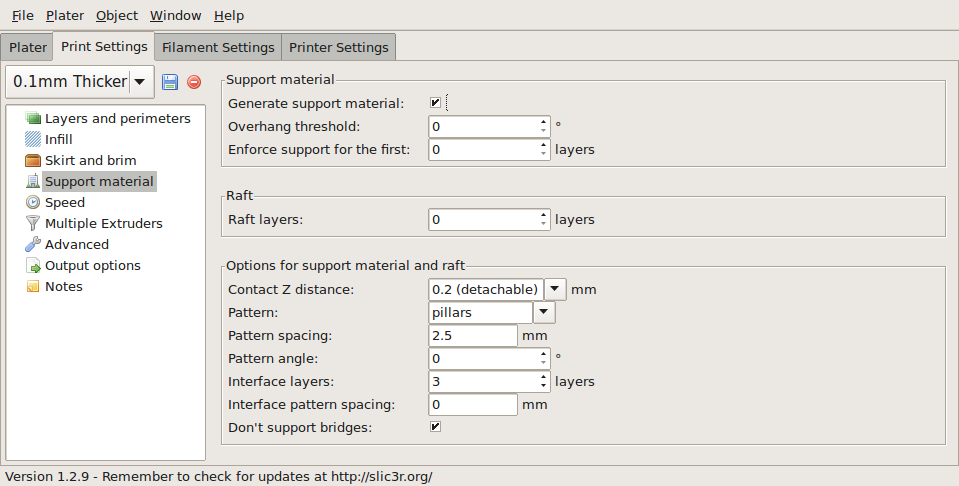
\includegraphics[keepaspectratio=true,width=1\textwidth]{expertmode/support/advanced_support.png}
\caption{Support structure options.}
\label{fig:advanced_support}
\end{figure}

The first thing to do is activate the support material option by checking the \texttt{Generate support material} box.  Providing a value of zero to the \texttt{Overhang threshold} parameter tells Slic3r to detect places to provide support automatically, otherwise the degrees given will be used.  Support generation is a relatively complex topic, and there are several aspects which determine the optimal support, it is strongly recommended to set the threshold to zero and allow Slic3r to determine the support required.

Small models, and those with small footprints, can sometimes break or detach from the bed.  Therefore the \texttt{Enforce support} option will cause support structures to be printed for the given number of layers, regardless of the angle threshold value.

To demonstrate the infill patterns the minimug model was tilted by 45° along the x axis, as shown in figure \ref{fig:support_minimug_45deg}.

\begin{figure}[H]
\centering
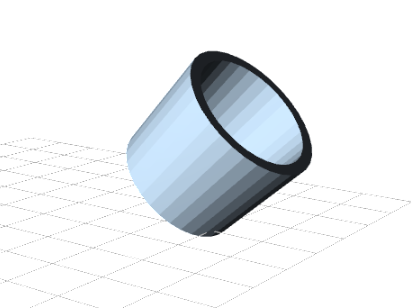
\includegraphics[keepaspectratio=true,width=0.75\textwidth]{expertmode/support/support_minimug_45deg.png}
\caption{Minimug model, tilted 45°.}
\label{fig:support_minimug_45deg}
\end{figure}

As with infill, there are several patterns available for the support structure.

\begin{figure}[H]
\centering
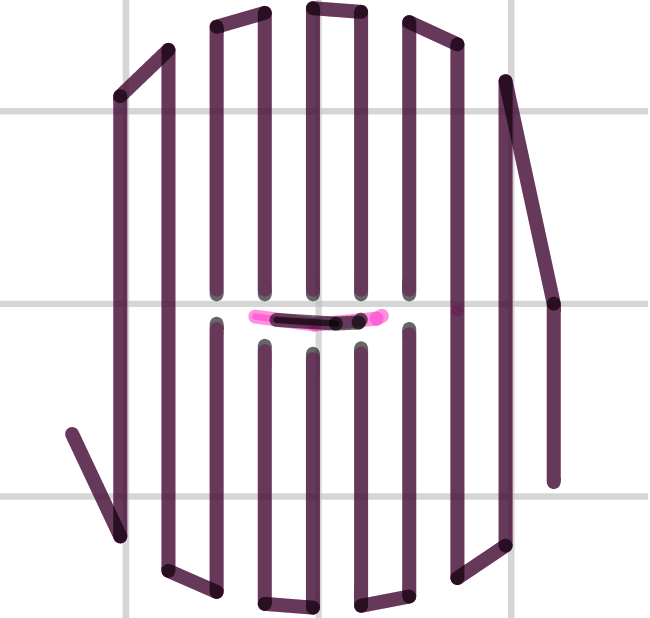
\includegraphics[keepaspectratio=true,width=0.2\textwidth]{expertmode/support/support_pattern_rectlinear.png}
\caption{Support infill pattern: Rectilinear}
\label{fig:support_pattern_rectlinear}
\end{figure}

\begin{figure}[H]
\centering
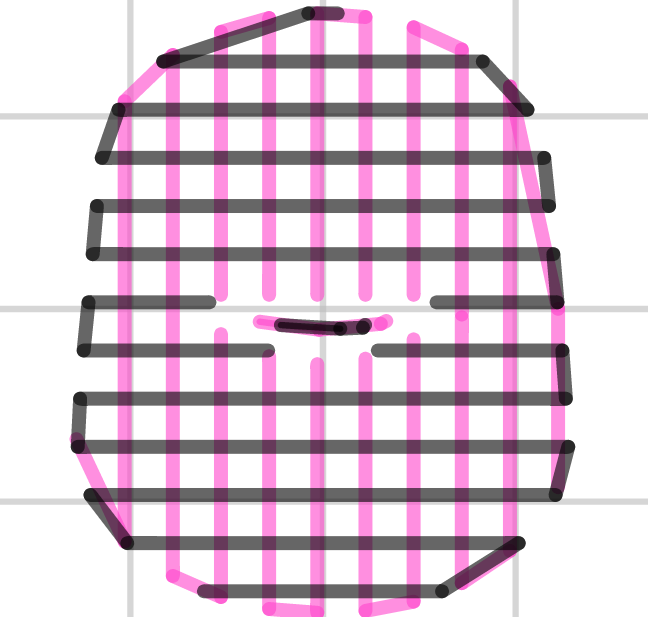
\includegraphics[keepaspectratio=true,width=0.2\textwidth]{expertmode/support/support_pattern_rectlinear_grid.png}
\caption{Support infill pattern: Rectilinear Grid}
\label{fig:support_pattern_rectlinear_grid}
\end{figure}

\begin{figure}[H]
\centering
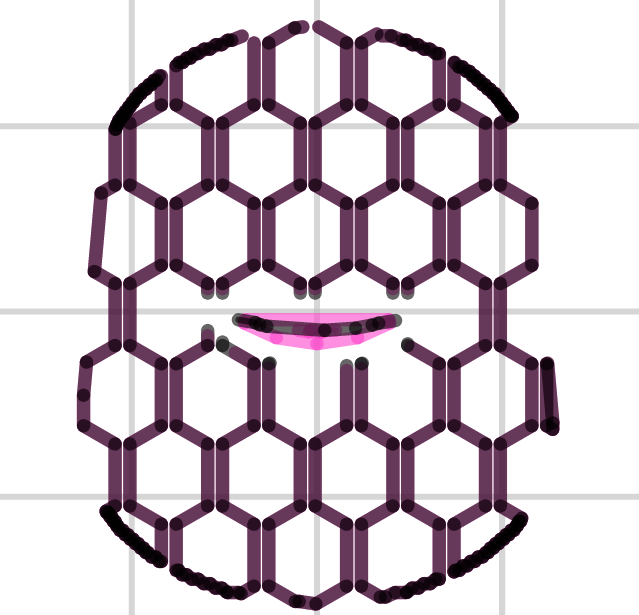
\includegraphics[keepaspectratio=true,width=0.2\textwidth]{expertmode/support/support_pattern_honeycomb.png}
\caption{Support infill pattern: Honeycomb}
\label{fig:support_pattern_honeycomb}
\end{figure}

\texttt{Pattern Spacing} determines the distance between support lines, and is akin to infill density apart from being defined only in mm.  If changing this attribute take into account the width of the support extrusion and the amount of support material that will adhere to the object.

Care should be taken to choose a support pattern which matches the model, where the support material attaches perpendicularly to the wall of the object, rather than in parallel, so it will be easy to remove.  If the support structure does run along the length of a wall then the \texttt{Pattern Angle} option allows the direction of the support lines to be rotated.

\begin{figure}[H]
\centering
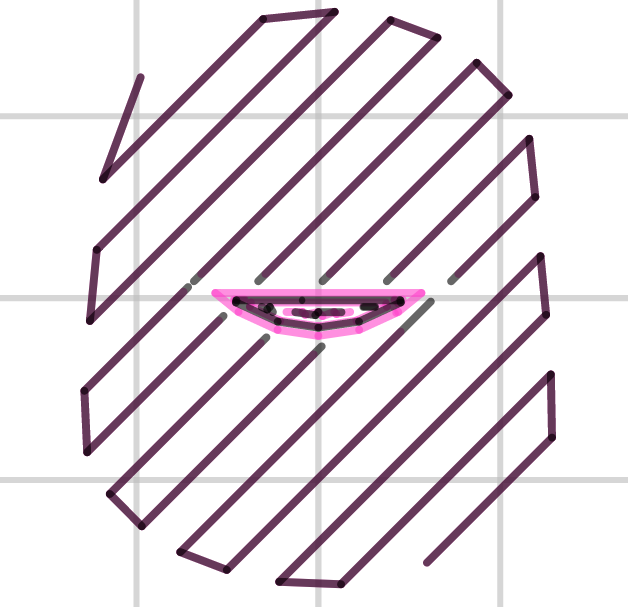
\includegraphics[keepaspectratio=true,width=0.2\textwidth]{expertmode/support/support_pattern_rectlinear_rotated.png}
\caption{Example of pattern angle rotated 45°.}
\label{fig:support_pattern_rectlinear_rotated}
\end{figure}


%TODO: Interface layers.


% section support (end)